% =========================================================
% main.tex (root file)
% =========================================================

\documentclass[masterthesis]{fer}
% Add the option upload to generate the final version which is uploaded to FERWeb
% Dodaj opciju upload za generiranje konačne verzije koja se učitava na FERWeb

\usepackage{blindtext}
\usepackage{float}

\usepackage{siunitx}
\sisetup{
  group-separator = {,},
  group-minimum-digits = 4
}


%--- THESIS INFORMATION / PODACI O RADU ----------------------------------------
\title{Deep learning-based animal re-identification for non-invasive wildlife monitoring and conservation}
\naslov{Duboko učenje za ponovnu identifikaciju životinja u neinvazivnom praćenju divljih vrsta i očuvanju prirode}
\author{Matej Marić}
\mentor{izv. prof. dr. sc. Marina Bagić Babac}
\date{June, 2025}
\datum{lipanj, 2025.}
%-------------------------------------------------------------------------------

\begin{document}

% Title page
\maketitle

% Thesis assignment sheet (download from FERWeb)
\zadatak{filename.pdf}

% Acknowledgements -----------------------------------------
\begin{zahvale}
Thanks for the tea...
\end{zahvale}

% Numbered pages from here
\mainmatter


% Table of contents (add \listoffigures or \listoftables if needed)
\tableofcontents

% ------------------------------------------------------------
% Include chapter files (kept in ./chapters/)
% ------------------------------------------------------------
\chapter{Introduction}
\label{chap:introduction}
The conservation and effective management of wildlife populations depend crucially on accurate methods for monitoring animal abundance and diversity. Traditional approaches, including manual identification, tagging are often invasive, costly, time-consuming and impractical at large scales or in remote environments. In recent years, significant progress has been achieved through the application of automated computer vision methods for wildlife monitoring, particularly though individual animal re-identification (Re-ID). Animal Re-ID, which refers to the task of identifying and matching individual animals across multiple observations solely on visual appearance, has emerged as a viable non-invasive method for ecological studies and conservation efforts.\cite{re-id-overview} Despite the advancements, current visual Re-ID systems still face substantial challenges, especially when applied to real-world scenarios characterized by significant appearance variations, environmental clutter, occlusions, and limited training data. Current methods typically require extensive manual labeling effort or species-specific model training, restricting their applicability in general ecological monitoring and conservation task so developing an efficient, flexible Re-ID framework capable of generalizing to virtually any animal species without requiring significant manual annotation or retraining represents an important and currently unmet need in conservation technology. The main aim of this thesis is just that, to develop a generalizable, robust animal Re-ID and population estimation system capable of performing reliably across diverse animal species with minimal manual intervention. Specifically, this thesis attempts to create a method suitable for real-world scenarios characterized by limited labeled data, eliminating the requirement for extensive manual labeling which can often be very difficult and error-prone cause it requires a certain expertise. To achieve these goals, the research was structured around two interlinked objectives:

\begin{enumerate}
    \item \textbf{Evaluation and optimization of robust classification methodologies}: Before addressing the complex task of population estimation, it was essential to establish a strong foundation for animal Re-ID that generalizes effectively across species. Publicly available datasets, notably WildlifeReID-10k \cite{adam2025wildlifereid10k}, were leveraged for evaluation and testing. This phase involved extensive experimentation with robust feature extraction methods, including DISK \cite{tyszkiewicz2020disklearninglocalfeatures} and LightGlue \cite{lindenberger2023lightgluelocalfeaturematching} combined with dimensionality reduction and aggregation approaches such as PCA, GMM and Fisher Vectors.
    \item \textbf{Development of population size estimation method: } Following the establishment of a reliable and generalizable individual classification framework, the ultimate goal was population counting. Implementatin of the Nested Importance Sampling (NIS)\cite{perez2024humanintheloopvisualreidpopulation}, a human-in-the-loop statistical framework leveraging pairwise similarity scores produced by the general-purpose Re-ID model. Critically, this method requires minimal human input and does not require additional training or extensive labeling for new animal species or datasets, thus significantly reduicng manual labor and expertise requirements in practical scenarios. Several potential week points were discovered in the paper itself which were attempted to address in this thesis. 
\end{enumerate}

All experiments and analyses in this thesis are conducted on publicly available datasets, primarily through the WildlifeReID-10k benchmark \cite{adam2025wildlifereid10k}, in order to support reproducible evaluation and fair comparisons across methods.

\chapter{Related Work}
\label{chap:related_work}
In this chapter, I will go over existing approaches to visual animal re-identification (Re-ID) with an emphasis on methods intended to generalize across species. The literature will be organized into thematic categories, from traditional computer vision techniques to modern deep learning methods, including hybrid methods that combine the two. I'll also discuss key challenges in the field, such as limited and/or low quality data, pose variation and open-set identification. I'll synthesize the findings from prior work and emphasize the gaps that this thesis is trying to address.

\section{Traditional Computer Vision Approaches}
Early animal Re-ID systems relied on hand-crafted visual features and local descriptors. A prime example is HotSpotter~\cite{6475023}, a SIFT-based~\cite{Lowe2004SIFT} algorithm that identifies individuals by comparing local keypoints in images. HotSpotter uses viewpoint-invariant SIFT descriptors and scores matches by emphasizing the most distinctive keypoints (the titular "hot spots") on an animal's coat pattern. ~\cite{jmse11050889} compared SIFT, SURF and SuperPoint on identifying sunfish individuals and demonstrated that the number of matching keypoints between a pair of images is a strong indicator for the likelihood that they contain the same individual. These traditional local-feature methods do not require training on identity labels and are, by definition, species-agnostic, making them applicable to a wide variety of species. HotSpotter and similar algorithms have been successfully used on numerous species with distinctive markings, including zebras, giraffes, jaguars, ocelots and leopards.~\cite{springerSpeciesAgnosticPatterned} The drawback, however, is that purely hand-crafted methods cannot fully exploit any available training data since their matching heuristic is fixed and may miss more subtle or global cues. 

\section{Species-Specific Trait-Based Re-Identification}
Another line of research focuses on species-specific visual traits for re-identification. Instead of analyzing the entire image or generic local patches, these approaches isolate particular biometric features unique to the species at hand, for example the ear shapes of elephants, the outline of a shark's dorsal fin, or the contour of a whale's tail (fluke), and use them for re-identification. Both traditional image analysis and deep learning have been employed to recognize such traits. For example, algorithms such as CurvRank~\cite{ani12151980} and finFindR~\cite{finFindR} compute and match the shapes of whale flukes or shark fins to identify individuals. These methods often don't require individual identity labels for training, rather a detector or feature extractor for the trait can be trained using only that trait's annotations, then match those features between images. The advantage of trait-specific methods is that they leverage highly distinctive features (when they are present) and can work with minimal ID labeling. However, a major limitation is that they are species-specific so each system is tailored for identifying only one species and usually it can't be transferred to other species. This lack of generality is a significant barrier to wider use as it requires developing a new method for each studied species. This thesis is motivated by overcoming this limitation by developing a method, based on existing research, that does not depend on any single species' unique traits. 

\section{Deep Learning-Based Methods}
With the rise of deep learning, a number of methods have been proposed that learn features directly from image data, without manual feature engineering. Modern deep learning approaches for animal re-ID typically employ CNNs (Convolutional Neural Networks) or related architectures to produce an embedding (feature vector) for each image, such that images of the same individual are close in feature space while those of different individuals are far apart. These can be trained either as classification (training a CNN to classify a fixed set of known individuals) or via metric learning (training the network to differentiate between same-individual vs. different individual image pairs). In general, metric learning approaches are favored for wildlife re-ID because they naturally handle open-set problems. A classification-based model treats re-ID as identifying one of $N$ known individuals, which fails when a new individual outside the training set appears. By contrast, metric-based methods learn a similarity function and can thus match new individuals by embedding comparison, without needing to retrain for new identities.~\cite{springerSpeciesAgnosticPatterned} Recent progress in this area has been accelerated by large-scale multidataset training and more standardized benchmarking. The WildlifeDatasets toolkit~\cite{čermák2023wildlifedatasetsopensourcetoolkitanimal} provides an easy and unified access to a wide array of re-ID datasets, enabling reproducible evaluation across species. MegaDescriptor is a model trained on these datasets that out-of-the-box provides a strong backbone for re-ID tasks. At the same time, large-scale training introduced an evaluation pitfall that is not discussed enough in the literature and that is excessive data leakage due to appearance of near-duplicates in the datasets. 

\section{Hybrid Approaches with Learned Local Features}
A promising direction in animal re-id is to combine the strengths of traditional and deep learning methods into a hybrid pipeline. The idea is to use modern learned features from deep networks in place of the hand-crafted ones, but still employ them in a local matching and aggregation framework as in traditional approaches. A good example of this is the ALFRE-ID~\cite{springerSpeciesAgnosticPatterned} pipeline (Aggregated Local Features for Re-Identification). ALFRE-ID uses a CNN extractor to extract local patch descriptors from an animal's coat pattern, then aggregates these local features into a global descriptor for the image. 

WildFusion~\cite{cermak2024wildfusionindividualanimalidentification} takes a different approach by combining global deep similarity and local matching similarity using calibration to make these scores comparable. Their results have shown that calibrated fusion can substantially improve accuracy across diverse benchmarks. The trade-off is computational cost, which motivated this thesis to create a faster system while preserving accuracy. 

\section{Population Estimation}
Individual identification is something that lends itself naturally to the task of estimating animal populations. Perez et al~\cite{perez2024humanintheloopvisualreidpopulation} propose Human-in-the-Loop Importance Sampling (HITL-NIS), an estimator grounded in statistics that queries a human annotator for a relatively small number of same/different pair judgements to estimate the number of individuals without fully clustering the dataset. However, human annotation is never perfect and Johansson et al.~\cite{Johansson_Samelius_Wikberg_Chapron_Mishra_Low_2020} show that identification errors in camera trap workflows can drastically bias population estimates, emphasizing the need to account for human mistakes. This thesis directly builds on this gap by evaluating HITL-NIS under simulated annotation noise to judge the robustness of the system. 



\section{Key Challenges and Limitations}
Research in animal re-identification encounters several fundamental challenges that limit real-world performance. Key issues identified in the literature are: 

  \textbf{Limited labeled data.} Collecting individual-level labels is
   labor-intensive, so datasets often contain only a handful of images per
   subject, leading to overfitting and poor generalization.  

   \textbf{Pose variation.} Animals appear under diverse viewpoints and
   behaviors, drastically altering their visual features. Identification
   accuracy drops when profiles or unusual poses replace frontal views.  

   \textbf{Occlusions.} Vegetation, group interactions, or partial camera trap
   captures often conceal distinguishing markings, hindering feature extraction.

   \textbf{Open-set identification.} Field deployments must handle individuals
   unseen during training; closed-set models misclassify such cases. Open-set
   recognition methods highlight the need to reject unknown identities.


\chapter{Datasets}
\label{chap:dataset}
Accurate and generalizable animal re-identification (Re-ID) system depends on the quality and diversity of datasets used for development and evaluation. This thesis evaluates the proposed approach on publicly available datasets, mostly from WildlifeReID-10k dataset collection\cite{adam2025wildlifereid10kwildlifereidentificationdataset}

\section{WildlifeReID-10k}
WildlifeReID-10k\cite{adam2025wildlifereid10kwildlifereidentificationdataset} is a benchmark dataset collection explicitly curated for evaluating animal Re-ID methods across a variety of species. The primary goal of this dataset is to enable systematic benchmarking of general-purpose animal Re-ID methods. It aggregates \num{37} existing datasets into a unified format to enable easy evaluation. In total, WildlifeReID contains \num{140488} images of \num{10772} unique individuals spanning \num{33} species. The methods described in this thesis were tested on \num{7} datasets from that collection: ATRW (tigers), CowDataset (cows), ElPephants (elephants), CTai (chimps), Chicks4FreeID (chickens), SealID (seals) and SeaStarReID2023 (sea stars). They were chosen because they provide the range of challenges of re-identification and the testing on all \num{37} datasets would be too computationally expensive.  

\begin{figure}[H]
    \centering
    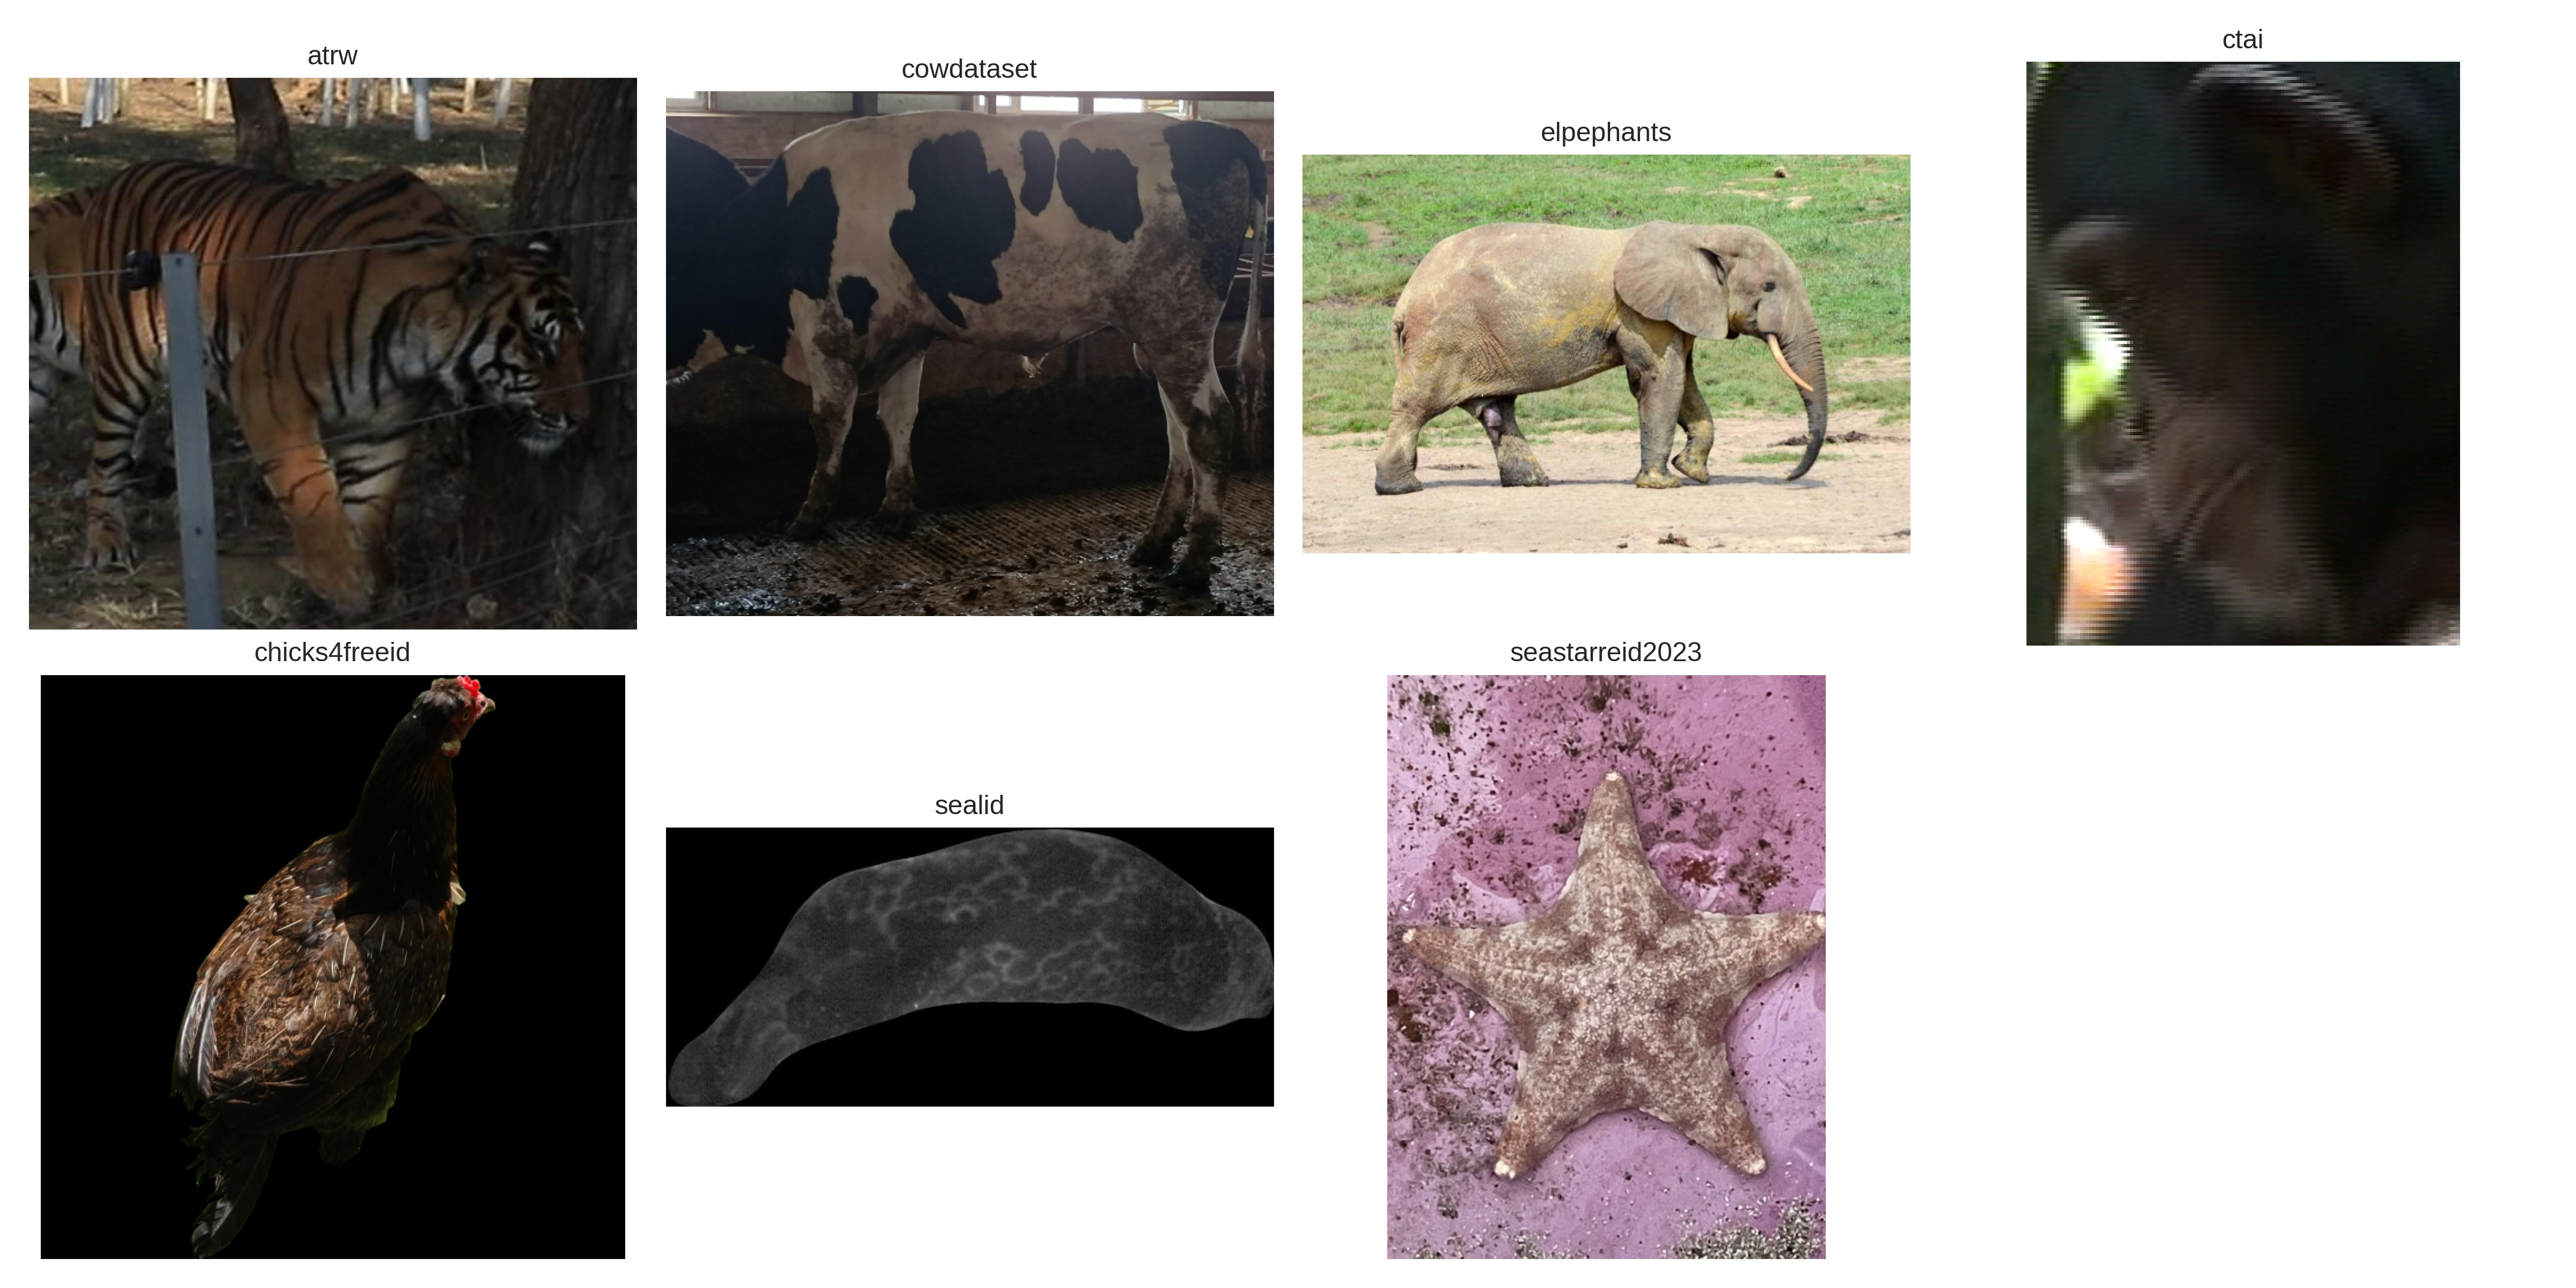
\includegraphics[width=0.95\linewidth]{Figures/dataset_examples_grid.JPG}
    \caption{Example images from the datasets used in this thesis.}
    \label{fig:dataset_examples_grid}
\end{figure}

\subsection{Train/Test Leakage Issues and Split Protocols}
A central (and often not addressed) issue in animal Re-ID evaluation is train-to-test leakage caused by visually almost identical images (for example, consecutive video frames or images from camera traps taken in very quick succession during a single observation) ending up in both train and test sets. There are also mistakes in the datasets, so in some cases there are literal duplicates present. Because of this random splits often result in overly optimistic results that do not reflect real-world generalization.\cite{adam2025wildlifereid10kwildlifereidentificationdataset}

To address this, WildlifeReID-10k proposes two split strategies\cite{adam2025wildlifereid10kwildlifereidentificationdataset}:

\begin{itemize}
    \item \textbf{Time-aware splits}: some of the datasets come with timestamps and this is used to split the images chronologically per identity using a cut-off date so that images from the same encounter do not leak across splits
    \item \textbf{Similarity-aware splits}: when timestamps are not available, an embedding model DINOv2\cite{oquab2024dinov2learningrobustvisual} is used to cluster the images, leveraging the fact that near duplicates should lie close in the embedding space
\end{itemize}

\subsection{MegaDescriptor Training Leakage}
In this thesis I used the MegaDescriptor-L-384 (MD) model for extracting of global embeddings from images, this model was trained on a subset of datasets from WildlifeReID-10k so for those datasets in evaluation I disregarded the time-aware/similarity-aware splits and used the exact same splits that the model was trained on to avoid additional data leaks. Those datasets are: ATRW, CTai and SealID and in later parts of the thesis will be marked with \textbf{*} to signify this. The Exception to this is the ELPephants\cite{Korschens_2019_ICCV} dataset which uses a random split.

\subsection{Datasets Overview}
\begin{table}[H]
\centering
\begin{tabular}{l r r r l}
\hline
\textbf{Dataset} & \textbf{\# images} & \textbf{\# individuals} & \textbf{ratio} & \textbf{split type}\\
\hline
ATRW* & 5,415 & 182 & 29.8 & Original MD split \\
CTai* & 4,662 & 71 & 65.7 & Original MD split \\
SealID* & 2,080 & 57 & 36.5 & Original MD split \\
CowDataset & 1,485 & 13 & 114.2 & Time-aware split \\
Chicks4FreeID & 1,146 & 50 & 22.9 & Similarity-aware split \\
SeaStarReID2023 & 2,187 & 95 & 23.0 & Time-aware split \\
ELPephants & 2078 & 276 & 7.5 & Random split \\
\hline
\end{tabular}
\caption{Datasets used for evaluation in this thesis.}
\label{tab:datasets_used}
\end{table}

\subsection{Class balance visualizations}
Another issue with Re-ID datasets is that they are typically highly imbalanced.

\begin{figure}[H]
    \centering
    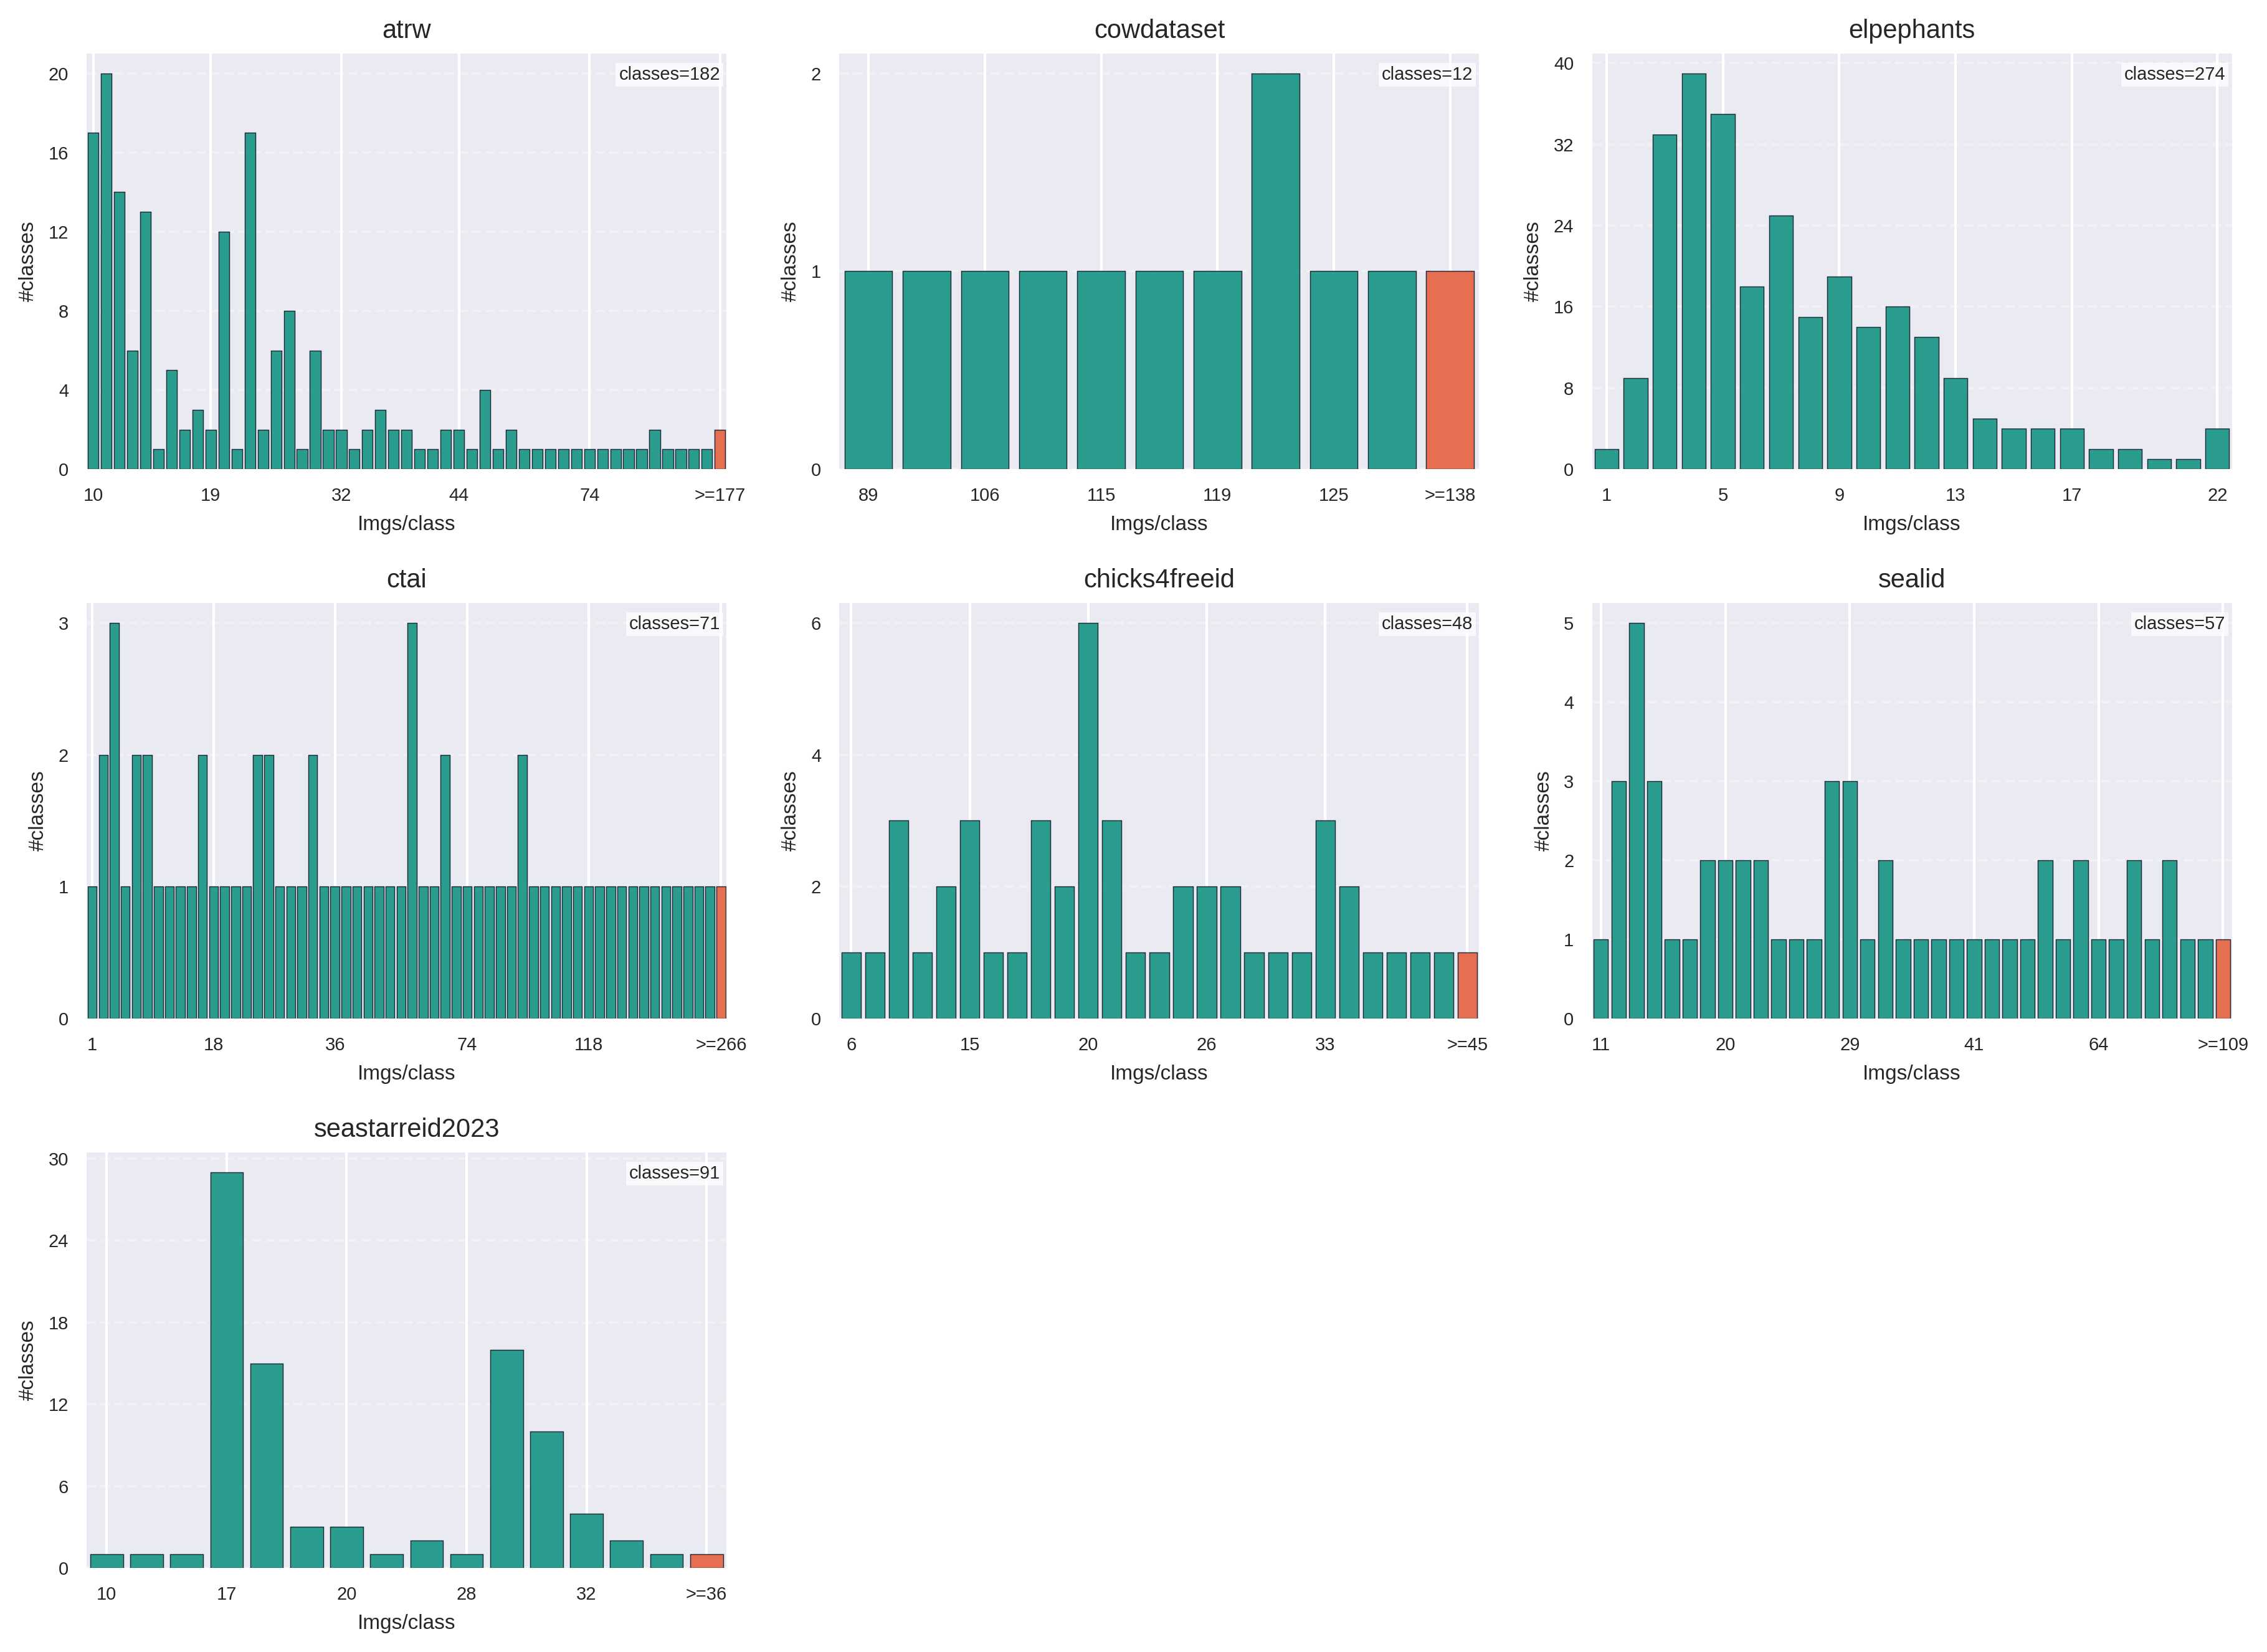
\includegraphics[width=0.95\linewidth]{Figures/class_balance_compact_grid.png}
    \caption{Class balance (number of images per individual) for the datasets used.}
    \label{fig:class_balance_compact_grid}
\end{figure}


\chapter{Methodology}
\label{chap:methodology}

This chapter describes the core stages of the proposed animal re-identification pipeline, used in both the classifcation mode and counting mode: preprocessing, feature extraction (global and local), aggregation of local descriptors into Fisher vectors (FV) and geometric verification used as an additional consistency check and for scoring.


\section{Preprocessing}
Wildlife images are rarely captured under controlled conditions, illumination can vary significantly, there can be backgroud clutter and/or occlusion. Preprocessing is used to reduce the variation and potential background bias.

\subsection{Mantiuk Tone Mapping}
Tone mapping compresses the dynamic range and enhances local contrast, making subtle patterns on the animal body more visible. Following the recommendation in \cite{springerSpeciesAgnosticPatterned}, this thesis uses Mantiuk tone mapping as an optional preprocessing step.

\subsection{Segmentation with Grounded SAM2}
Even if the images in a dataset are cropped, backgroud can still dominate local or global feature extraction which can lead to background bias. To eliminate this effect, a segmentation-based pipeline is used to isolate the animal from the background. The pipeline first localizes the animal using a text prompted dectector (GroundingDINO)\cite{groundingdino} and then produces a pixel level mask using Segment Anything Model 2 (SAM2)\cite{ravi2024sam2}. The mask is applied with soft edges to avoid introducing shart boundaries that could create non-existent keypoints.

\begin{figure}[H]
    \centering
    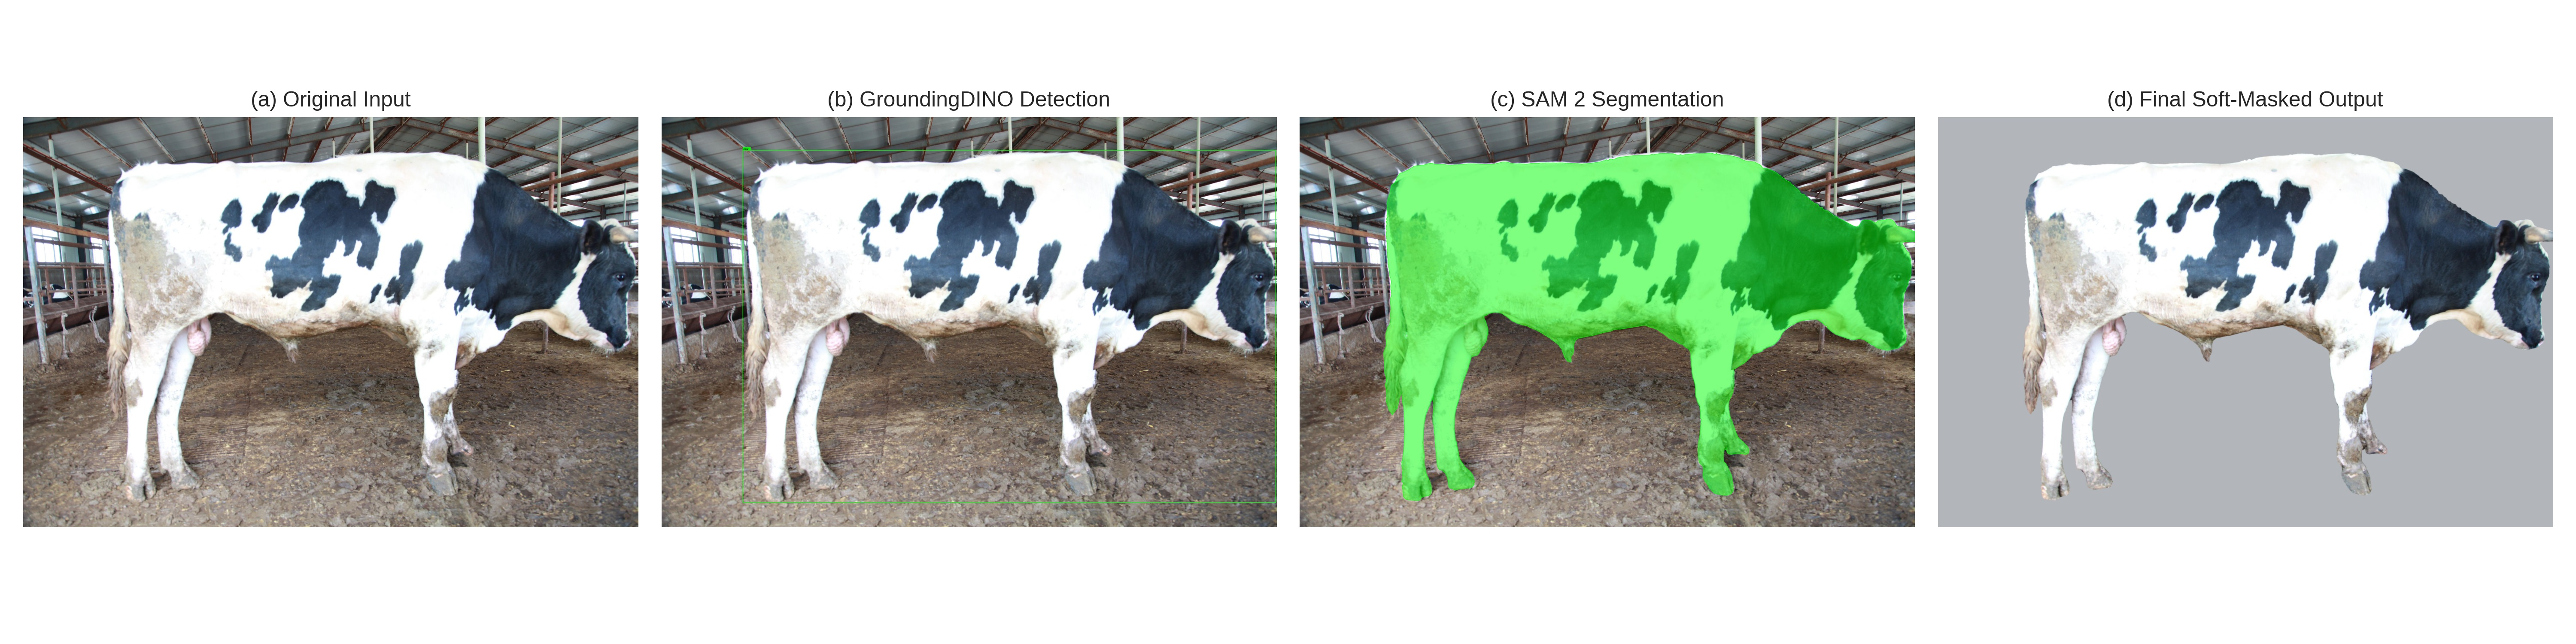
\includegraphics[width=0.95\linewidth]{Figures/segmentation_pipeline_vis.JPG}
    \caption{Overview of the segmentation-based preprocessing pipeline used for background removal.}
    \label{fig:segmentation_pipeline}
\end{figure}

Segmentation was not applied to all datasets in this thesis since some already came segmented or, in case of CTai, were already cropped so tightly that it was deemed unnecessary. 

\section{Feature Extraction}
\label{sec:feature_extraction}
Feature extraction is a critical component of animal Re-Identification pipelines, converting raw image data into a representation that can be compared across observations. This thesis uses two complementary families of features: global embeddings and local features.

\subsection{Why combine global and local features?}
Global embeddings summarize the entire image into a single vector and provide a fast, strong retrieval signal. Local features, on the other hand, represent an image as a set of keypoints and descriptors, which can capture fine-grained details and allow geometric consistency checks. These two feature families are evaluated both independently and in combination in later experiments.

\subsection{Global Embeddings}
\label{subsec:global_embeddings}

Global embeddings are a fixed-length feature vector produced by a pre-trained neural network (MD). Two images can then be compared by measuring the distance or similarity between their embeddings (in this thesis, cosine similarity is used).

For global embeddings, I used MegaDescriptor-L-384\cite{čermák2023wildlifedatasetsopensourcetoolkitanimal}, a large Swin Transformer model trained specifically for animal re-identification. It was trained on 29 publicly available datasets from WildlifeDatasets collection\cite{čermák2023wildlifedatasetsopensourcetoolkitanimal}. This provides a strong baseline similarity signal that is efficient and fast to compute and can be fused with the results of local methods.\cite{cermak2024wildfusionindividualanimalidentification}

\subsection{Local Features}
\label{subsec:local_feature_detection}
Local features model an image as a set of keypoints and associated descriptors. Matching local features between two images can give a similarity signal and also enables geometric verification. In practice, this is a two-step process: first keypoints are detected, and then each keypoint is described with a feature vector.

In this thesis, I used three modern learning-based local feature extractors:
SuperPoint\cite{DeTone2018SuperPoint}, DISK\cite{tyszkiewicz2020disklearninglocalfeatures},
and ALIKED\cite{zhao2023alikedlighterkeypointdescriptor}. Although each method performs
well individually, experiments showed that they are complementary, so they were also used
as an ensemble. These methods were selected because they work well out-of-the-box without
dataset-specific fine-tuning, while learning-based local features generally provide stronger
matching performance than classical handcrafted alternatives such as SIFT\cite{Lowe2004SIFT}.

Once keypoints are detected, we compute descriptors that summarize the appearance of the local region around each keypoint. An effective descriptor should be discriminative (distinguishing one region from another) and robust (invariant to geometric transformations).

\subsubsection{SuperPoint}
SuperPoint\cite{DeTone2018SuperPoint} uses a single convolutional network with two heads:
one predicts interest-point scores and the other predicts dense local descriptors.
It is trained in a self-supervised manner using synthetic homographic warps, which encourages
both detector repeatability and descriptor consistency under viewpoint changes.

\subsubsection{DISK}
DISK (DIScrete Keypoints)\cite{tyszkiewicz2020disklearninglocalfeatures} is an end-to-end
trainable framework that jointly learns keypoint detection and description. Its training
objective directly optimizes matching quality across image pairs, making it well suited for
retrieval and re-identification settings where reliable correspondence is required.

\subsubsection{ALIKED}
ALIKED\cite{zhao2023alikedlighterkeypointdescriptor} is a lightweight learned detector-descriptor
model designed for efficient local feature extraction. It uses a deformable transformation
strategy to better adapt to geometric variation while keeping inference computationally practical.
In this thesis, ALIKED provides a strong speed-accuracy trade-off and complements SuperPoint and
DISK in the ensemble setting.


\subsection{Local Matching}
Local descriptors are compared by matching keypoints between images. In this thesis, matching is performed with LightGlue\cite{lindenberger2023lightgluelocalfeaturematching}. Concretely, for each image pair LightGlue is provided with the extracted keypoint coordinates and their descriptors (from SuperPoint/DISK/ALIKED) and it outputs a set of tentative matches (index pairs of matching keypoints). We then use those matches as input to geometric verification (Section~\ref{sec:geometric_verification}).

\begin{figure}[H]
    \centering
    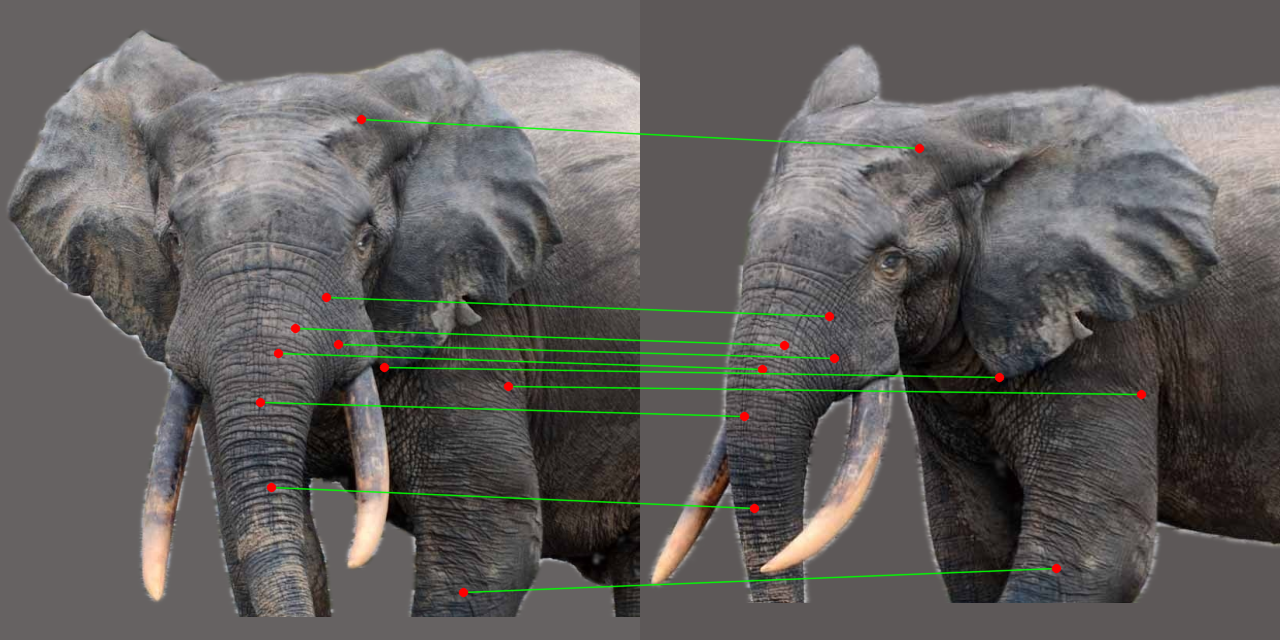
\includegraphics[width=0.95\linewidth]{Figures/visualize_matches.png}
    \caption{Example local feature matches between two images with backgrounds removed. Limited to 10 keypoints for visual clarity.}
    \label{fig:visualize_matches}
\end{figure}

\section{Feature Aggregation and Representation}
\label{sec:feature_aggregation}
Local feature matching is powerful but computationally expensive when comparing many query images against a large database. To enable efficient large-scale comparison, this thesis also aggregates sets of local descriptors into a single fixed-length representation using Fisher Vectors (FV)\cite{5540009}. The FV representation is built on PCA (Principal Component Analysis) for dimensionality reduction and GMM (Gaussian Mixture Model) that servers as a visual vocabulary\cite{springerSpeciesAgnosticPatterned}.


\subsection{Training PCA and GMM models}
\label{sec:pca_gmm_training}

Feature descriptors extracted from images can be high-dimensional and noisy. Thus, dimensionality reduction and normalization are performed to improve efficiency and accuracy.

Initially PCA is applied to decorrelate and reduce the dimensionality of the descriptors. PCA projects the original descriptors onto a lower-dimensional subspace defined by the principal eigenvectors of the covariance matrix computed from the descriptors. This is also important later on for the computation of fisher vectors because they produce very large descriptors.\cite{springerSpeciesAgnosticPatterned}

After dimensionality reduction, a Gaussian Mixture Model (GMM) is trained on the reduced descriptors. A GMM models the descriptor distribution as a weighted sum of $K$ Gaussian components, each parameterized by mean vectors $\{\mu_k\}$, covariance matrices $\{\Sigma_k\}$, and weights $\{\pi_k\}$. Specifically, a GMM is defined as:
\begin{equation}
    p(x) = \sum_{k=1}^{K}\pi_k \mathcal{N}(x|\mu_k,\Sigma_k),
\end{equation}

where $\mathcal{N}(x|\mu_k,\Sigma_k)$ denotes the probability density function of the $k$-th Gaussian component. This codebook (the trained GMM) captures the visual vocabulary and statistical distribution of the reduced descriptors from the training images.\cite{springerSpeciesAgnosticPatterned}

In simpler terms, PCA finds the directions in which the descriptor values vary the most and keeps only those, so each feature becomes a shorter, uncorrelated vector that is faster to store and compare. Then we model how these compact vectors are distributed. GMM model assumes that the whole set of vectors can be grouped into a number of smooth clusters, each cluster described by it's mean, spread and relative weight in the mixture. Together, these clusters form a codebook meaning that every new descriptor can be represented as a weighted combination of the nearest clusters, giving us both a compressed encoding and a way to compute similarity for matching or classification which is of crucial importance in re-identification task. 

\subsection{Fisher Vector Computation}
\label{sec:fisher_vector_computation}
Fisher vectors (FV) are an image representation technique that captures statistical deviations of local features from a visual vocabulary (codebook) modeled by GMM. FV measures how features differ from typical patterns in a reference GMM and they encode both first-order differences (mean shifts) and second-order differences (variance changes) in feature distribution. The output is a high-dimensional vector that acts as a "signature" of an image's unique feature distribution. Basically, given a set of descriptors extracted from a single image, FV encodes how these descriptors deviate from the trained GMM parameters. Fisher Vectors represent the gradients of the log-likelihood function with respect to the GMM parameters. Formally, given an image with descriptors $X = \{x_t\}_{t=1}^{T}$ where $\lambda$ is a vector of GMM parameters and $u_\lambda$ is a probability density function modeling the distribution of the data. 

This gradient is formally knows as the score function\cite{springerSpeciesAgnosticPatterned}. It measures the sensitivity of the log-likelihood to changes in the model parameters, essentially indicating how to adjust the GMM to better fit the observed features. 

\begin{equation}
G_\lambda^X = L_\lambda \log u_\lambda(X),
\end{equation}

When constructing a FV for an image, a set of local features is assumed to be independent which means that the final descriptor can be constructed as a sum of Fisher Vectors for each local feature:\cite{springerSpeciesAgnosticPatterned}

\begin{equation}
G{_\lambda^{X}} = \sum_{t = 1}^{T} L_{\lambda} \nabla_{\lambda} \log u_{\lambda}(x_t)
\end{equation}

The matrix $L_\lambda$ is derived from the Fisher Information Matrix and is used to "whiten" or to normalize the gradients\cite{article}, making them more discriminative and suitable for use in classification later on.

Following the standard practice, this vector is computed separately for means and variances, resulting in a final vector of dimension $2KD$, where $K$ is the number of Gaussian components and $D$ the dimensionality of the PCA-reduced descriptors. L2 and power normalization have also been applied since they have been shown\cite{10.1007/978-3-642-15561-1_11} to generally improve the performance of the method.

FV have also been chosen because they have been shown to perform better that bag-of-words approaches.\cite{5540009}

\subsection{Parameter Choices and Rationale}
\label{sec:parameter_choices}

Several key parameters influenced the effectiveness of Fisher Vectors for the re-identification task during the development:

\begin{itemize}
    \item \textbf{Number of PCA components ($N_{PCA}$):} A balance between dimensionality reduction and retention of discriminative information.
    \item \textbf{Number of GMM components ($N_{GMM}$):} Controls the granularity of the visual codebook. More components typically yield richer representations but increase computational complexity.
\end{itemize}

These parameters were empirically determined based on experimenting and computational constraints. Specifically, the PCA dimension was selected to retain approximately 95\% of descriptor variance. The number of GMM components was chosen to balance accuracy and computational efficiency. The best results were achieved, with $96$ PCA components, $256$ GMM components.

\section{Geometric Verification}
\label{sec:geometric_verification}
Geometric verification is used to make sure that matched keypoints between images truly correspond to the same physical locations on an animal reducing false positives that arise from visual similarites alone. This step is crucial in refining the initial matches obtained through descriptor-based feature matching by enforcing spatial consistency.\cite{springerSpeciesAgnosticPatterned}

\subsection{Theoretical Foundation}
Local feature descriptors such as DISK\cite{tyszkiewicz2020disklearninglocalfeatures} or KeyNet combined with AffNet and HardNet \cite{keynet, mishkin2018repeatabilityenoughlearningaffine, Mishchuk2017HardNet}, offer robust initial matches based on visual similarity. However, matches that are generated purely from descriptor similarity may include mistakes, especially in visually cluttered or repetitive environments common in wildlife images. Geometric verification, as suggested in \cite{springerSpeciesAgnosticPatterned}, addresses this by validating matches through spatial coherence checks. 

\subsection{Establishing Initial Correspondences}
Initial correspondences are established trough descriptor matching using LightGlue\cite{lindenberger2023lightgluelocalfeaturematching}, an attention-based method. Initially methods like Lowe's ratio test were considered but matching with LightGlue proved significantly faster and more accurate, effectively eliminating the need for traditional filtering methods.

\subsection{Transformation Estimation}
The core of GV involves estimating a homography transformation between matched keypoints using RANSAC (Random Sample Consensus). RANSAC iteratively samples minimal subsets of correspondences, computes candidate transformations and evaluates their agreement with the remaining matches. Matches that fall within a defined spatial threshold are considered inliers. 

\subsection{Scoring and Verification}
Matches are assessed primarily by their inlier count, the number of matches consistent with the estimated homography, and their spatial distribution:

    \begin{itemize}
        \item \textbf{Inlier count:} Number of correspondences that agree with the estimated transformation; higher counts suggest more reliable matches.
        \item \textbf{Inlier ration: } Normalizes the inlier count by the total number of tentative matches,
  $$
  r = \frac{|I|}{|C|},
  $$
  where $|I|$ denotes the inlier count and $|C|$ the total correspondences.
        \item \textbf{Combined scoring:} Integrates geometric consistency with descriptor similarity (fisher vector distances or global distances) to leverage both spatial and appearance information.
    \end{itemize}
Penalties for low inlier counts or poor geometric coherence discourage accepting borderline matches, improving the overall system reliability and accuracy.

%\chapter{Feature Aggregation and Representation}
\label{chap:feature_aggregation}
This chapter describes the process of aggregating local feature descriptors extracted from animal images into compact global representations suitable for efficient comparison and re-identification. As described in \cite{springerSpeciesAgnosticPatterned} Fisher Vectors (FV) were utilized, built on PCA and Gaussian Mixture Models (GMMs).

\section{Training PCA and GMM models}
\label{sec:pca_gmm_training}

Feature descriptors extracted from images can be high-dimensional and noisy. Thus, dimensionality reduction and normalization are performed to improve efficiency and accuracy.

Initially PCA is applied to decorrelate and reduce the dimensionality of the descriptors. PCA projects the original descriptors onto a lower-dimensional subspace defined by the principal eigenvectors of the covariance matrix computed from the descriptors. This is also important later on for the computation of fisher vectors because they produce very large descriptors.\cite{springerSpeciesAgnosticPatterned}

After dimensionality reduction, a Gaussian Mixture Model (GMM) is trained on the reduced descriptors. A GMM models the descriptor distribution as a weighted sum of $K$ Gaussian components, each parameterized by mean vectors $\{\mu_k\}$, covariance matrices $\{\Sigma_k\}$, and weights $\{\pi_k\}$. Specifically, a GMM is defined as:
\begin{equation}
    p(x) = \sum_{k=1}^{K}\pi_k \mathcal{N}(x|\mu_k,\Sigma_k),
\end{equation}

where $\mathcal{N}(x|\mu_k,\Sigma_k)$ denotes the probability density function of the $k$-th Gaussian component. This codebook (the trained GMM) captures the visual vocabulary and statistical distribution of the reduced descriptors from the training images.\cite{springerSpeciesAgnosticPatterned}

In simpler terms, PCA finds the directions in which the descriptor values vary the most and keeps only those, so each feature becomes a shorter, uncorrelated vector that is faster to store and compare. Then we model how these compact vectors are distributed. GMM model assumes that the whole set of vectors can be grouped into a number of smooth clusters, each cluster described by it's mean, spread and relative weight in the mixture. Together, these clusters form a codebook meaning that every new descriptor can be represented as a weighted combination of the nearest clusters, giving us both a compressed encoding and a way to compute similarity for matching or classification which is of crucial importance in re-identification task. 

\section{Fisher Vector Computation}
\label{sec:fisher_vector_computation}
Fisher vectors (FV) are an image representation technique that captures statistical deviations of local features from a visual vocabulary (codebook) modeled by GMM. FV measures how features differ from typical patterns in a reference GMM and they encode both first-order differences (mean shifts) and second-order differences (variance changes) in feature distribution. The output is a high-dimensional vector that acts as a "signature" of an image's unique feature distribution. Basically, given a set of descriptors extracted from a single image, FV encodes how these descriptors deviate from the trained GMM parameters. Fisher Vectors represent the gradients of the log-likelihood function with respect to the GMM parameters. Formally, given an image with descriptors $X = \{x_t\}_{t=1}^{T}$ where $\lambda$ is a vector of GMM parameters and $u_\lambda$ is a probability density function modeling the distribution of the data. 

This gradient is formally knows as the score function\cite{springerSpeciesAgnosticPatterned}. It measures the sensitivity of the log-likelihood to changes in the model parameters, essentially indicating how to adjust the GMM to better fit the observed features. 

\begin{equation}
G_\lambda^X = L_\lambda \log u_\lambda(X),
\end{equation}

When constructing a FV for an image, a set of local features is assumed to be independent which means that the final descriptor can be constructed as a sum of Fisher Vectors for each local feature:\cite{springerSpeciesAgnosticPatterned}

\begin{equation}
G{_\lambda^{X}} = \sum_{t = 1}^{T} L_{\lambda} \nabla_{\lambda} \log u_{\lambda}(x_t)
\end{equation}

The matrix $L_\lambda$ is derived from the Fisher Information Matrix and is used to "whiten" or to normalize the gradients\cite{article}, making them more discriminative and suitable for use in classification later on.

Following the standard practice, this vector is computed separately for means and variances, resulting in a final vector of dimension $2KD$, where $K$ is the number of Gaussian components and $D$ the dimensionality of the PCA-reduced descriptors. L2 and power normalization have also been applied since they have been shown\cite{10.1007/978-3-642-15561-1_11} to generally improve the performance of the method.

FV have also been chosen because they have been shown to perform better that bag-of-words approaches.\cite{5540009}

\section{Parameter Choices and Rationale}
\label{sec:parameter_choices}

Several key parameters influenced the effectiveness of Fisher Vectors for the re-identification task during the development:

\begin{itemize}
    \item \textbf{Number of PCA components ($N_{PCA}$):} A balance between dimensionality reduction and retention of discriminative information.
    \item \textbf{Number of GMM components ($N_{GMM}$):} Controls the granularity of the visual codebook. More components typically yield richer representations but increase computational complexity.
    \item \textbf{Maximum descriptors sampled ($MAX\_GMM\_DESCRIPTORS$):} Limits the number of descriptors sampled for training PCA and GMM to manage memory usage and computational load.
\end{itemize}

These parameters were empirically determined based on experimenting and computational constraints. Specifically, the PCA dimension was selected to retain approximately 95\% of descriptor variance. The number of GMM components was chosen to balance accuracy and computational efficiency. The best results were achieved, with $96$ PCA components, $256$ GMM components and $200,000$ descriptors. The larger number of maximal components could perhaps prove better results but computational constraints were a limiting factor.
%\chapter{Geometric Verification}
\label{chap:geometric_verification}
Geometric verification is used to make sure that matched keypoints between images truly correspond to the same physical locations on an animal reducing false positives that arise from visual similarites alone. This step is crucial in refining the initial matches obtained through descriptor-based feature matching by enforcing spatial consistency.

\section{Theoretical Foundation}
Local feature descriptors such as DISK\cite{tyszkiewicz2020disklearninglocalfeatures} or KeyNet combined with AffNet and HardNet \cite{keynet, mishkin2018repeatabilityenoughlearningaffine, Mishchuk2017HardNet}, offer robust initial matches based on visual similarity. However, matches that are generated purely from descriptor similarity may include mistakes, especially in visually cluttered or repetitive environments common in wildlife images. Geometric verification, as suggested in \cite{springerSpeciesAgnosticPatterned}, addresses this by validating matches through spatial coherence checks. 

\section{Establishing Initial Correspondences}
Initial correspondences are established trough descriptor matching using LightGlue\cite{lindenberger2023lightgluelocalfeaturematching}, an attention-based method. Initially methods like Lowe's ratio test were considered but matching with LightGlue proved significantly faster and more accurate, effectively eliminating the need for traditional filtering methods.

\section{Transformation Estimation with RANSAC}
The core of geometric verification involves estimating a homography transformation between matched keypoints using RANSAC (Random Sample Consensus).RANSAC iteratively samples minimal subsets of correspondences, computes candidate transformations and evaluates their agreement with the remaining matches. Matches that fall within a defined spatial threshold are considered inliers. 

\section{Scoring and Verification}
Matches are assessed primarily by their inlier count, the number of matches consistent with the estimated homography, and their spatial distribution:

    \begin{itemize}
        \item \textbf{Inlier count:} Number of correspondences that agree with the estimated transformation; higher counts suggest more reliable matches.
        \item \textbf{Inlier ration: } Normalizes the inlier count by the total number of tentative matches,
  $$
  r = \frac{|I|}{|C|},
  $$
  where $|I|$ denotes the inlier count and $|C|$ the total correspondences.
        \item \textbf{Combined scoring:} Integrates geometric consistency with descriptor similarity (fisher vector distances) to leverage both spatial and appearance information.
    \end{itemize}
Penalties for low inlier counts or poor geometric coherence discourage accepting borderline matches, improving the overall system reliability and accuracy.

\chapter{Classification}
Here we will describe in detail the process of classification
\chapter{Population Size Estimation}

Here I will, in detail, describe hte process of population counting.

\section{Introduction}

While individual animal re-identification provides the foundation for wildlife monitoring, the ultimate goal in many conservation and ecological applications is estimating population sizes. Traditional clustering approaches for population estimation often produce inaccurate results when applied to re-identification systems, particularly when the underlying pairwise similarities are noisy or unreliable~\cite{perez2024humanintheloopvisualreidpopulation}.

In this chapter I present the implementation and adaptation of Nested Importance Sampling (NIS) for population size estimation, originally proposed by Perez et al.~\cite{perez2024humanintheloopvisualreidpopulation}. The method provides a statistically principled approach to estimate the number of unique individuals in a dataset by leveraging pairwise similarity scores from the re-identification system developed in previous chapters. Critically, this work extends the original framework by implementing a fully automated variant that eliminates the need for human annotation during the estimation process.

\section{Theoretical Foundation}

\subsection{Population Size as Connected Components}

The population estimation problem can be formulated as counting connected components in a graph where vertices represent images and edges exist between images of the same individual. Formally, given a graph $G = (V, E)$ where vertices correspond to images and edges represent same-individual relationships, the number of clusters $K$ equals the number of connected components:

\begin{equation}
K = \text{CC}(G) = \sum_{u=1}^{n} \frac{1}{1 + d(u)}
\label{eq:connected_components}
\end{equation}

where $d(u)$ is the degree of vertex $u$ (i.e., the number of edges connected to $u$)~\cite{perez2024humanintheloopvisualreidpopulation}.

This elegant formulation arises from the observation that the graph $G$ consists of a collection of cliques, where each clique represents images of the same individual. The clique containing vertex $u$ has size $1 + d(u)$, and the total contribution of all vertices in this clique is $(1 + d(u)) \times \frac{1}{1 + d(u)} = 1$. Thus, each clique contributes exactly 1 to the sum, yielding the total number of connected components.

This formulation provides the foundation for statistical estimation: instead of computing all pairwise similarities explicitly, we can sample vertices and estimate their degrees, then use importance sampling to obtain an unbiased estimate of the population size.

\subsection{Nested Importance Sampling Framework}

The NIS framework operates through a two-stage sampling process designed to efficiently estimate the population size while minimizing the number of pairwise comparisons required:

\begin{enumerate}
\item \textbf{Outer sampling}: Sample $N$ vertices from the graph according to a proposal distribution $Q(u) \propto \frac{1}{1 + \hat{d}(u)}$, where $\hat{d}(u)$ is the estimated degree based on approximate pairwise similarities.

\item \textbf{Inner sampling}: For each sampled vertex $u_i$, sample $M$ neighbors according to $q_{u_i}(v) \propto \hat{s}(u_i, v)$, where $\hat{s}(u, v)$ is the approximate similarity between images $u$ and $v$.
\end{enumerate}

The population estimate is then computed as:

\begin{equation}
\widehat{\text{CC}}_{\text{NIS}}(G) = \frac{1}{N} \sum_{i=1}^{N} \frac{1}{Q(u_i)} \times \frac{1}{1 + \hat{d}(u_i)}
\label{eq:nis_estimator}
\end{equation}

where $\hat{d}(u_i)$ is estimated through the inner sampling process~\cite{perez2024human}.

The key insight behind this approach is that the proposal distribution $Q(u)$ biases sampling towards isolated vertices (those with low degrees), as these contribute most significantly to the cluster count. Similarly, the inner sampling distribution biases towards sampling nodes that are likely to be connected, maximizing the information gained from each pairwise query.

\section{Automated Adaptation with Geometric Verification}

\subsection{Motivation for Automation}

The original NIS framework relies on human annotation to verify whether pairs of images contain the same individual~\cite{perez2024humanintheloopvisualreidpopulation}. While this approach provides high accuracy, it presents practical limitations for large-scale deployments where manual annotation becomes prohibitively expensive or where expert annotators are unavailable. To address these limitations, this work develops a fully automated variant that leverages geometric verification as described in Chapter~\ref{chap:geometric_verification}.

\subsection{Similarity Computation}

The approximate pairwise similarities $\hat{s}(u,v)$ are derived from the fused Fisher vector representations computed in the feature aggregation stage (Chapter~\ref{chap:feature_aggregation}). Cosine similarity is computed between normalized feature vectors and converted to a probability distribution using softmax normalization with temperature parameter $\tau = 0.5$:

\begin{equation}
\hat{s}(u,v) = \frac{e^{\hat{c}(u,v)/\tau}}{\sum_v e^{\hat{c}(u,v)/\tau}}
\end{equation}

where $\hat{c}(u,v) = \frac{\Phi(x_u) \cdot \Phi(x_v)}{||\Phi(x_u)||_2 ||\Phi(x_v)||_2}$ represents the normalized cosine similarity between feature vectors.

\subsection{Automated Verification Process}

Instead of relying on human verification of pairwise similarities, the automated system employs a gated verification process that combines Fisher vector distances with geometric verification. The process operates as follows:

\begin{enumerate}
\item \textbf{Initial filtering}: For each sampled pair $(u, v)$, verify that sufficient keypoints and descriptors are available for geometric verification.

\item \textbf{Geometric verification}: Apply the geometric verification pipeline (Chapter~\ref{chap:geometric_verification}) to compute geometric distance and inlier count.

\item \textbf{Confidence assessment}: Combine geometric quality metrics with Fisher vector similarity to produce an overall confidence score:

\begin{align}
\text{confidence} &= \min\left(1.0, \frac{n_{\text{inliers}}}{20.0}\right) \\
\text{geometric\_quality} &= 1.0 - d_{\text{geometric}} \\
\text{overall\_confidence} &= 0.6 \times \text{geometric\_quality} + 0.4 \times \text{confidence}
\end{align}

\item \textbf{Binary decision}: Accept the pair as a match if the overall confidence exceeds 0.5 and the number of inliers meets the minimum threshold.
\end{enumerate}

This automated approach eliminates the need for human annotation while maintaining the statistical framework of the original NIS method.

\section{Advantages and Limitations}

\subsection{Advantages}

The automated NIS approach offers several key advantages over traditional clustering methods:

\begin{enumerate}
\item \textbf{Statistical guarantees}: Unlike heuristic clustering approaches, the NIS framework provides asymptotically unbiased population estimates with confidence intervals, enabling principled uncertainty quantification.

\item \textbf{Minimal supervision}: The automated mode eliminates the need for human annotation during population estimation, making it practical for large-scale deployments where expert annotation is unavailable or prohibitively expensive.

\item \textbf{Robustness}: The method handles noisy pairwise similarities better than traditional clustering approaches by explicitly modeling uncertainty through the sampling framework.

\item \textbf{Scalability}: Computational complexity scales as $N \times M$ rather than $n^2$, where $N$ and $M$ are sampling parameters and $n$ is the total number of images, enabling application to large datasets.
\end{enumerate}

\subsection{Limitations and Bias Considerations}

The automated approach introduces several sources of bias that must be acknowledged:

\begin{enumerate}
\item \textbf{Geometric verification bias}: The reliance on geometric verification may systematically exclude certain types of valid matches, particularly:
\begin{itemize}
    \item Images with significant pose variations where keypoint correspondences are sparse
    \item Low-texture regions with insufficient keypoints for reliable geometric estimation
    \item Cases where the homography model is inappropriate for the underlying transformation
\end{itemize}

\item \textbf{Feature quality dependence}: The method's accuracy is fundamentally limited by the quality of the underlying Fisher vector representations and local feature extraction. Poor feature extraction can lead to both false positives and false negatives in the verification process.

\item \textbf{Threshold sensitivity}: The automated matching decisions depend on carefully tuned thresholds (geometric distance threshold, minimum inlier count, confidence threshold) that may not generalize across different species or imaging conditions.

\item \textbf{Systematic underestimation}: By requiring geometric consistency, the automated mode may systematically underestimate population sizes when valid matches are rejected due to overly restrictive geometric constraints. This represents a conservative bias that prioritizes precision over recall.
\end{enumerate}

\subsection{Bias-Variance Trade-off}

The automated approach represents a fundamental trade-off between bias and variance. While the original human-in-the-loop method provides nearly unbiased estimates (assuming perfect human annotation), it requires substantial manual effort. The automated variant introduces systematic bias through the geometric verification gate but enables deployment at scale without human intervention.

This trade-off is particularly relevant in conservation applications where obtaining population estimates—even if slightly biased—may be more valuable than having no estimates at all due to the prohibitive cost of manual annotation.

\section{Parameter Configuration}

The implementation includes several key parameters that influence the bias-variance trade-off:

\begin{itemize}
\item \textbf{$N$ (n\_vertices)}: Number of vertices sampled in the outer loop (default: 100)
\item \textbf{$M$ (n\_neighbors)}: Number of neighbors sampled per vertex (default: 10) 
\item \textbf{$\theta$ (gv\_threshold)}: Distance threshold for geometric verification acceptance (default: 0.75)
\item \textbf{$I_{\min}$ (min\_inliers)}: Minimum number of RANSAC inliers required for acceptance
\end{itemize}

These parameters represent a trade-off between computational efficiency and estimation accuracy. Higher sampling rates ($N$, $M$) generally produce more reliable estimates at increased computational cost, while more restrictive geometric thresholds ($\theta$, $I_{\min}$) reduce false positive matches but may increase systematic underestimation bias.

\section{Integration with the Re-ID Pipeline}

The population estimation module integrates seamlessly with the re-identification pipeline developed in previous chapters:

\begin{enumerate}
\item \textbf{Input}: Fused feature representations from the feature aggregation stage (Chapter~\ref{chap:feature_aggregation})
\item \textbf{Optional inputs}: Keypoints and descriptors for geometric verification (Chapter~\ref{chap:geometric_verification})
\item \textbf{Processing}: NIS-based sampling and automated verification
\item \textbf{Output}: Population estimate with standard error and detailed verification statistics
\end{enumerate}

This integration allows the system to provide both individual re-identification capabilities and population-level statistics from the same underlying feature representations, maximizing the utility of the computational pipeline.

\section{Summary}

This chapter presented the implementation of automated population size estimation using Nested Importance Sampling. The approach extends the original human-in-the-loop framework~\cite{perez2024humanintheloopvisualreidpopulation} by replacing human annotation with geometric verification, enabling fully automated deployment while maintaining the statistical rigor of the importance sampling framework.

While the automated approach introduces systematic bias through the geometric verification gate, it provides a practical solution for large-scale population estimation where human annotation is unavailable or prohibitively expensive. The method's effectiveness is evaluated experimentally in the following chapters, with particular attention to quantifying the trade-offs between automation and accuracy across different animal species and imaging conditions.



%\chapter{Pipeline Implementation}
\label{chap:pipeline}
This chapter details the practical implementation of the entire animal re-identification pipeline, connecting feature extraction, feature aggregation, geometric verification, and the classification components into a complete end-to-end workflow. It provides insight into the project's architecture, optimization strategies and computational considerations.

\section{System Overview}
\label{sec:system_overview}

The implemented pipeline consist of sequential, interconnected stages:

\begin{enumerate}
    \item \textbf{Image acquisition and pre-processing}
    \item \textbf{Segmentation}
    \item \textbf{Local feature extraction and description}
    \item \textbf{Feature aggregation (Fisher Vector computation)}
    \item  \textbf{Similarity retrieval and geometric verification}
\end{enumerate}

 The theory most of this we covered in the preceeding chapters so here we'll go indepth about how each component was implemented. The architecture itself was mostly inspired by the ALFRE-ID system describerd in \cite{springerSpeciesAgnosticPatterned} with some modifications and additions in an effort to improve on it.

 Figure~\ref{fig:pipeline_overview} Za ovdje napraviti sliku koja vizualizira cijeli pipeline.

\section{Software Architecture}
\label{sec:software_architecture}

The implementation is done entirely in Python, leveraging popular libraries for efficiency and reproducibility:

\begin{itemize}
    \item \textbf{PyTorch} for deep-learning based methods (local feature extraction).
    \item \textbf{OpenCV} for image processing and pre-processing tasks.
    \item \textbf{scikit-learn} for PCA and GMM training.
    \item \textbf{NumPy and SciPy} for numerical computations.
    \item \textbf{h5py} for efficient storage and retrieval of large descriptor datasets.
\end{itemize}

The codebase is modular, enabling easy experimentation and component swapping.

\section{Implementation of Feature Extraction Methods}
\label{sec:implementation_feature_extraction}

Two (? Ovo možda naraste na 3) primary feature extraction pipelines were implemented:

\subsection{DISK-based Extraction}
\begin{enumerate}
    \item Load the pre-trained DISK model \cite{tyszkiewicz2020disklearninglocalfeatures}.
    \item Images are resized to $640\times640$ pixels and converted to grayscale.
    \item Keypoints and descriptors are directly computed by a single forward pass.
    \item Store resulting descriptors and keypoints efficiently.
\end{enumerate}

\subsection{KeyNet-AffNet-HardNet Extraction}
Instead of DISK, a combination of KeyNet-AffNet-HardNet can be used for feature extraction, this method, as we will discuss in the later chapters proved to deliver slightly better results than DISK on most datasets tested, but was also slower and more memory intensive. 

\begin{enumerate}
    \item Extract initial keypoints with KeyNet \cite{Barroso2019KeyNet}.
    \item AffNet\cite{mishkin2018repeatabilityenoughlearningaffine} performs local affine normalization of detected patches.
    \item Generate descriptors from normalized patches using HardNet \cite{Mishchuk2017HardNet}.
    \item Descriptors and keypoints are stored separately in HDF5 files for downstream tasks.
\end{enumerate}

For memory purposes, the number of keypoints is capped at $5000$, this number was selected as a tradeoff between speed, accuracy and memory limitations.
\section{Feature Aggregation Implementation}
\label{sec:fv_implementation}

Feature descriptors are aggregated using PCA and GMM-based Fisher Vector representation (described previously in Chapter~\ref{sec:fisher_vector_computation}). Practical considerations in the implementation include:
\begin{enumerate}
    \item \textbf{Descriptor Sampling:} Random sampling of descriptors to manage computational complexity.
    \item \textbf{PCA Training:} PCA~\cite{sklearn_api} reduces dimensionality and applies whitening.
    \item \textbf{GMM Training:} A Gaussian Mixture Model (GMM)~\cite{sklearn_api} with diagonal covariance is fitted to PCA-reduced descriptors.
    \item \textbf{Fisher Vector Computation:} Fisher vectors encode gradients of log-likelihoods relative to trained GMM parameters.
\end{enumerate}

\section{Similarity Retrieval and Geometric Verification}
\label{sec:similarity_verification_implementation}

The retrieval component involves two key stages:

\begin{enumerate}
    \item \textbf{Initial retrieval:} Cosine similarity between Fisher Vectors rapidly identifies potential matches.
    \item \textbf{Geometric Verification:} Matches are further verified using RANSAC-based homography estimation (explained in detail in chapter XYZ
\end{enumerate}

The geometric verification implementation includes optimizations such as descriptor normalization and coordinate normalization to enhance RANSAC performance.

%\chapter{Experimental Setup}
\label{chap:experiments}

This chapter summarizes the experimental setup used to evaluate both the re-identification (classification) pipeline and the population counting module.

\section{Datasets and split protocols}
Experiments are conducted primarily on datasets from the WildlifeReID-10k collection~\cite{adam2025wildlifereid10kwildlifereidentificationdataset} as described in Chapter~\ref{chap:dataset}. When using MegaDescriptor-L-384 for global embeddings, we follow the split protocol discussed in Chapter~\ref{chap:dataset} to avoid train/test leakage on datasets that were part of the MegaDescriptor training set.

\section{Evaluation metrics}
\subsection{Classification (re-identification)}
For the closed-set identification task, we report:
\begin{itemize}
    \item \textbf{Top-1 accuracy}: fraction of queries whose predicted identity matches the ground truth.
    \item \textbf{Top-5 accuracy}: fraction of queries where the correct identity appears among the five most confident predictions.
    \item \textbf{F1 score}: reported for completeness as a balance of precision and recall under the per-query identity decision rule.
\end{itemize}

\subsection{Population counting}
For HITL-NIS, we report:
\begin{itemize}
    \item \textbf{Estimated population size} \(\widehat{K}\) and its \textbf{standard error} (and the derived confidence interval).
    \item \textbf{Oracle query diagnostics}: number of oracle calls and unique queried pairs.
    \item \textbf{Runtime}: wall-clock time for the sampling-and-oracle loop (excluding one-time feature extraction and calibration training).
\end{itemize}

\section{Runtime measurement}
Runtime values reported in Chapter~\ref{chap:results} correspond to the wall-clock time measured by the evaluation scripts. For the classification pipeline, this includes dataset loading and matching, and may include cached feature reuse depending on whether features were previously computed. For population counting, the reported runtime focuses on the HITL-NIS loop itself, as this is the component that scales with the number of oracle queries.
\chapter{Results}
\label{chap:results}
\begin{itemize}
    \item Rezultati klasifikacije (top-1, top-n acc), rezultati prebrojavanja individualnih životinja, rezultati prebrojavanja na mom datasetu
    \item Vizualizacije, tablice
    \item Usporedba utjecaja hiperparametara testiranih
\end{itemize}
%\chapter{Discussion}
\label{chap:discussion}
\begin{itemize}
    \item Interpretation of results.
    \item Successes and limitations.
    \item Comparison with related work.
\end{itemize}
\chapter{Conclusion and Future Work}
\label{chap:conclusion}
\begin{itemize}
    \item Summary of contributions and findings.
    \item Potential extensions and open questions.
\end{itemize}

% ----------------- References ------------------------------
\bibliography{references}

% ----------------- Abstract (EN) ---------------------------
\begin{abstract}
Reliable wildlife population monitoring is essential for conservation and ecological management. This thesis develops a species-agnostic visual pipeline that re-identifies individual animals and supports population size estimation when only limited labeled data is available. The method combines global deep embeddings with local-feature aggregation via Fisher vectors, and optionally applies geometric verification as a final re-ranking stage to improve robustness to viewpoint, background, and near-duplicate imagery. Evaluation is performed exclusively on publicly available benchmarks from the WildlifeReID-10k collection spanning multiple species and imaging conditions. Results show that fusing global and local evidence consistently improves closed-set identification performance, and that a human-in-the-loop nested importance sampling estimator can provide practical population estimates while highlighting sensitivity to labeling errors.
\end{abstract}

\begin{keywords}
Animal Re-identification; Wildlife Monitoring; Population Estimation; Computer Vision; Conservation
\end{keywords}

% ----------------- Sažetak (HR) -----------------------------
\begin{sazetak}
Pouzdano praćenje populacija divljih životinja ključno je za očuvanje prirode i ekološko upravljanje. U ovom radu razvijen je vizualni sustav neovisan o vrsti za re-identifikaciju pojedinačnih životinja i procjenu veličine populacije u uvjetima ograničene količine označenih podataka. Predloženi pristup kombinira globalne duboke ugrađene reprezentacije s agregacijom lokalnih značajki pomoću Fisherovih vektora te, po potrebi, primjenjuje geometrijsku verifikaciju kao završno ponovno rangiranje kako bi se povećala robusnost na promjene pogleda, pozadine i gotovo identične snimke. Evaluacija je provedena isključivo na javno dostupnim referentnim skupovima iz kolekcije WildlifeReID-10k koji obuhvaćaju više vrsta i različite uvjete snimanja. Rezultati pokazuju da fuzija globalnih i lokalnih signala dosljedno poboljšava uspješnost identifikacije, dok procjena populacije temeljena na interaktivnom ugniježđenom važnosnom uzorkovanju omogućuje praktične procjene uz naglašenu osjetljivost na pogreške u ljudskom označavanju.
\end{sazetak}

\begin{kljucnerijeci}
Re-identifikacija životinja; Nadzor Divljači; Procjena Populacije; Računalni Vid; Očuvanje Prirode
\end{kljucnerijeci}

\end{document}

